\documentclass[crop,tikz]{standalone}

\usepackage[utf8]{inputenc}
\usepackage{ifthen}
\usepackage{amsmath}

% 'crop' is the default for v1.0, before it was 'preview'
%\usetikzlibrary{...}% tikz package already loaded by 'tikz' option

\begin{document}

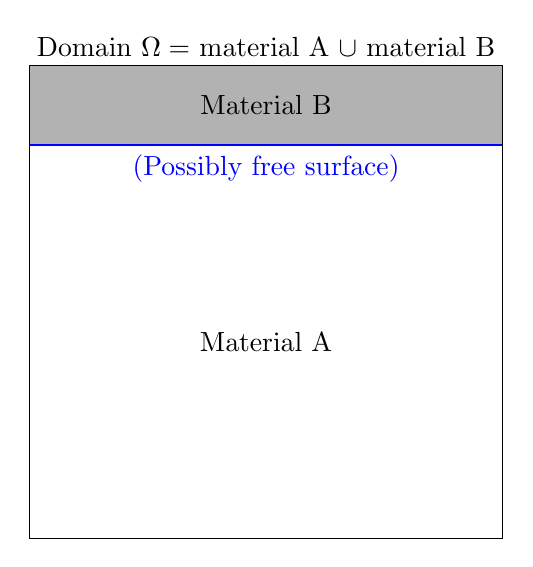
\begin{tikzpicture}

	\draw (-3,-3) rectangle (3,2);
	\draw[fill=black!30!white] (-3,2) rectangle (3,3);
	
	\node at (0,-0.5) {Material A};
	\node at (0,2.5) {Material B};
	\draw[thick, blue] (-3,2) -- (3,2);
	\node[anchor=north, blue] at (0,2) {(Possibly free surface)};
	
	\node[anchor=south] at (0,3) {Domain $\Omega = $ material A $\cup$ material B};
		
\end{tikzpicture}

\end{document}